\appendix

    \captionsetup{font={color=white}}

    \section{Flowchart}
    \begin{figure}[H] \centering
        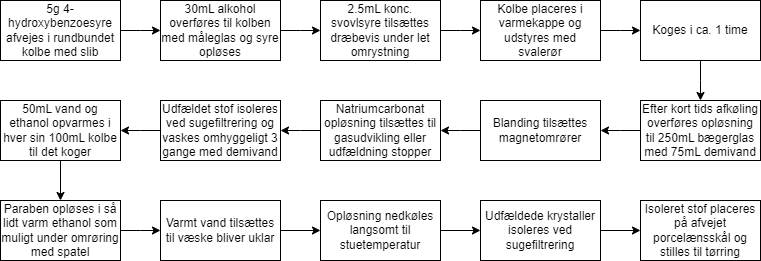
\includegraphics[width=\textwidth]{bilag/flowdiagram}
        \caption{}
    \end{figure} 
    
    \section{Mængdeberegninger}
    \subsection{Ethylparaben}
    \begin{table}[H]\centering
        \resizebox{\textwidth}{!}{
        \begin{tabular}{ccccc}
            \toprule
            Stof & Mængde $\left[\si{g} \vee \si{mL}\right]$ & Densitet $\left[\si{g\per mL}\right]$ & MV $\left[\si{g\per mol}\right]$ & Stofmængde $\left[\si{mol}\right]$ \\
            \midrule
            4-hydroxybenzoesyre & 5.1338 & & 138.12 & 0.0372 \\
            Ethanol & 30 & 0.79 & 46.07 & 0.514 \\
            Teoretisk ethylparaben & 5.66 & & & \\
            Praktisk ethylparaben & 2.2666 & & & \\
            \midrule
            Afvigelse & -60\% \\
            \bottomrule
        \end{tabular}
        }
        \caption{} \vskip -32pt
    \end{table}

    \subsection{Propylparaben}
    \begin{table}[H]\centering
        \resizebox{\textwidth}{!}{
        \begin{tabular}{ccccc}
            \toprule
            Stof & Mængde $\left[\si{g} \vee \si{mL}\right]$ & Densitet $\left[\si{g\per mL}\right]$ & MV $\left[\si{g\per mol}\right]$ & Stofmængde $\left[\si{mol}\right]$ \\
            \midrule
            4-hydroxybenzoesyre & 5.0346 & & 138.12 & 0.0365 \\
            Propanol & 30 & 0.803 & 60.1 & 0.401 \\
            Teoretisk propylparaben & 5.55 & & & \\
            Praktisk propylparaben & 4.4144 & & & \\
            \midrule
            Afvigelse & -20\% \\
            \bottomrule
        \end{tabular}
        }
        \caption{} \vskip -24pt
    \end{table}


    \subsection{Dobbeltsyntese}
    \begin{table}[H]\centering
        \resizebox{\textwidth}{!}{
        \begin{tabular}{ccccc}
            \toprule
            Stof & Mængde $\left[\si{g} \vee \si{mL}\right]$ & Densitet $\left[\si{g\per mL}\right]$ & MV $\left[\si{g\per mol}\right]$ & Stofmængde $\left[\si{mol}\right]$ \\
            \midrule
            4-hydroxybenzoesyre & 5.0176 & & 138.12 & 0.0363 \\
            Ethanol & 30 & 0.79 & 46.07 & 0.514 \\
            Teoretisk ethylparaben & 5.53 & & & \\
            Praktisk ethylparaben & 2.4244 & & & \\
            \midrule
            Afvigelse & -56\% \\
            \bottomrule
        \end{tabular}
        }
        \caption{} \vskip -12pt
    \end{table}
    
    \begin{table}[H]\centering
        \resizebox{\textwidth}{!}{
        \begin{tabular}{ccccc}
            \toprule
            Stof & Mængde $\left[\si{g} \vee \si{mL}\right]$ & Densitet $\left[\si{g\per mL}\right]$ & MV $\left[\si{g\per mol}\right]$ & Stofmængde $\left[\si{mol}\right]$ \\
            \midrule
            4-hydroxybenzoesyre & 5.0346 & & 138.12 & 0.0365 \\
            Propanol & 30 & 0.803 & 60.1 & 0.401 \\
            Teoretisk propylparaben & 5.55 & & & \\
            Praktisk propylparaben & 0.5692 & & & \\
            \midrule
            Afvigelse & -90\% \\
            \bottomrule
        \end{tabular}
        }
        \caption{} \vskip -24pt
    \end{table}
    
    \captionsetup{font={color=black}}
    \section{TLC--plader}
    \subsection{Syntese 1}
    \begin{figure}[H]
        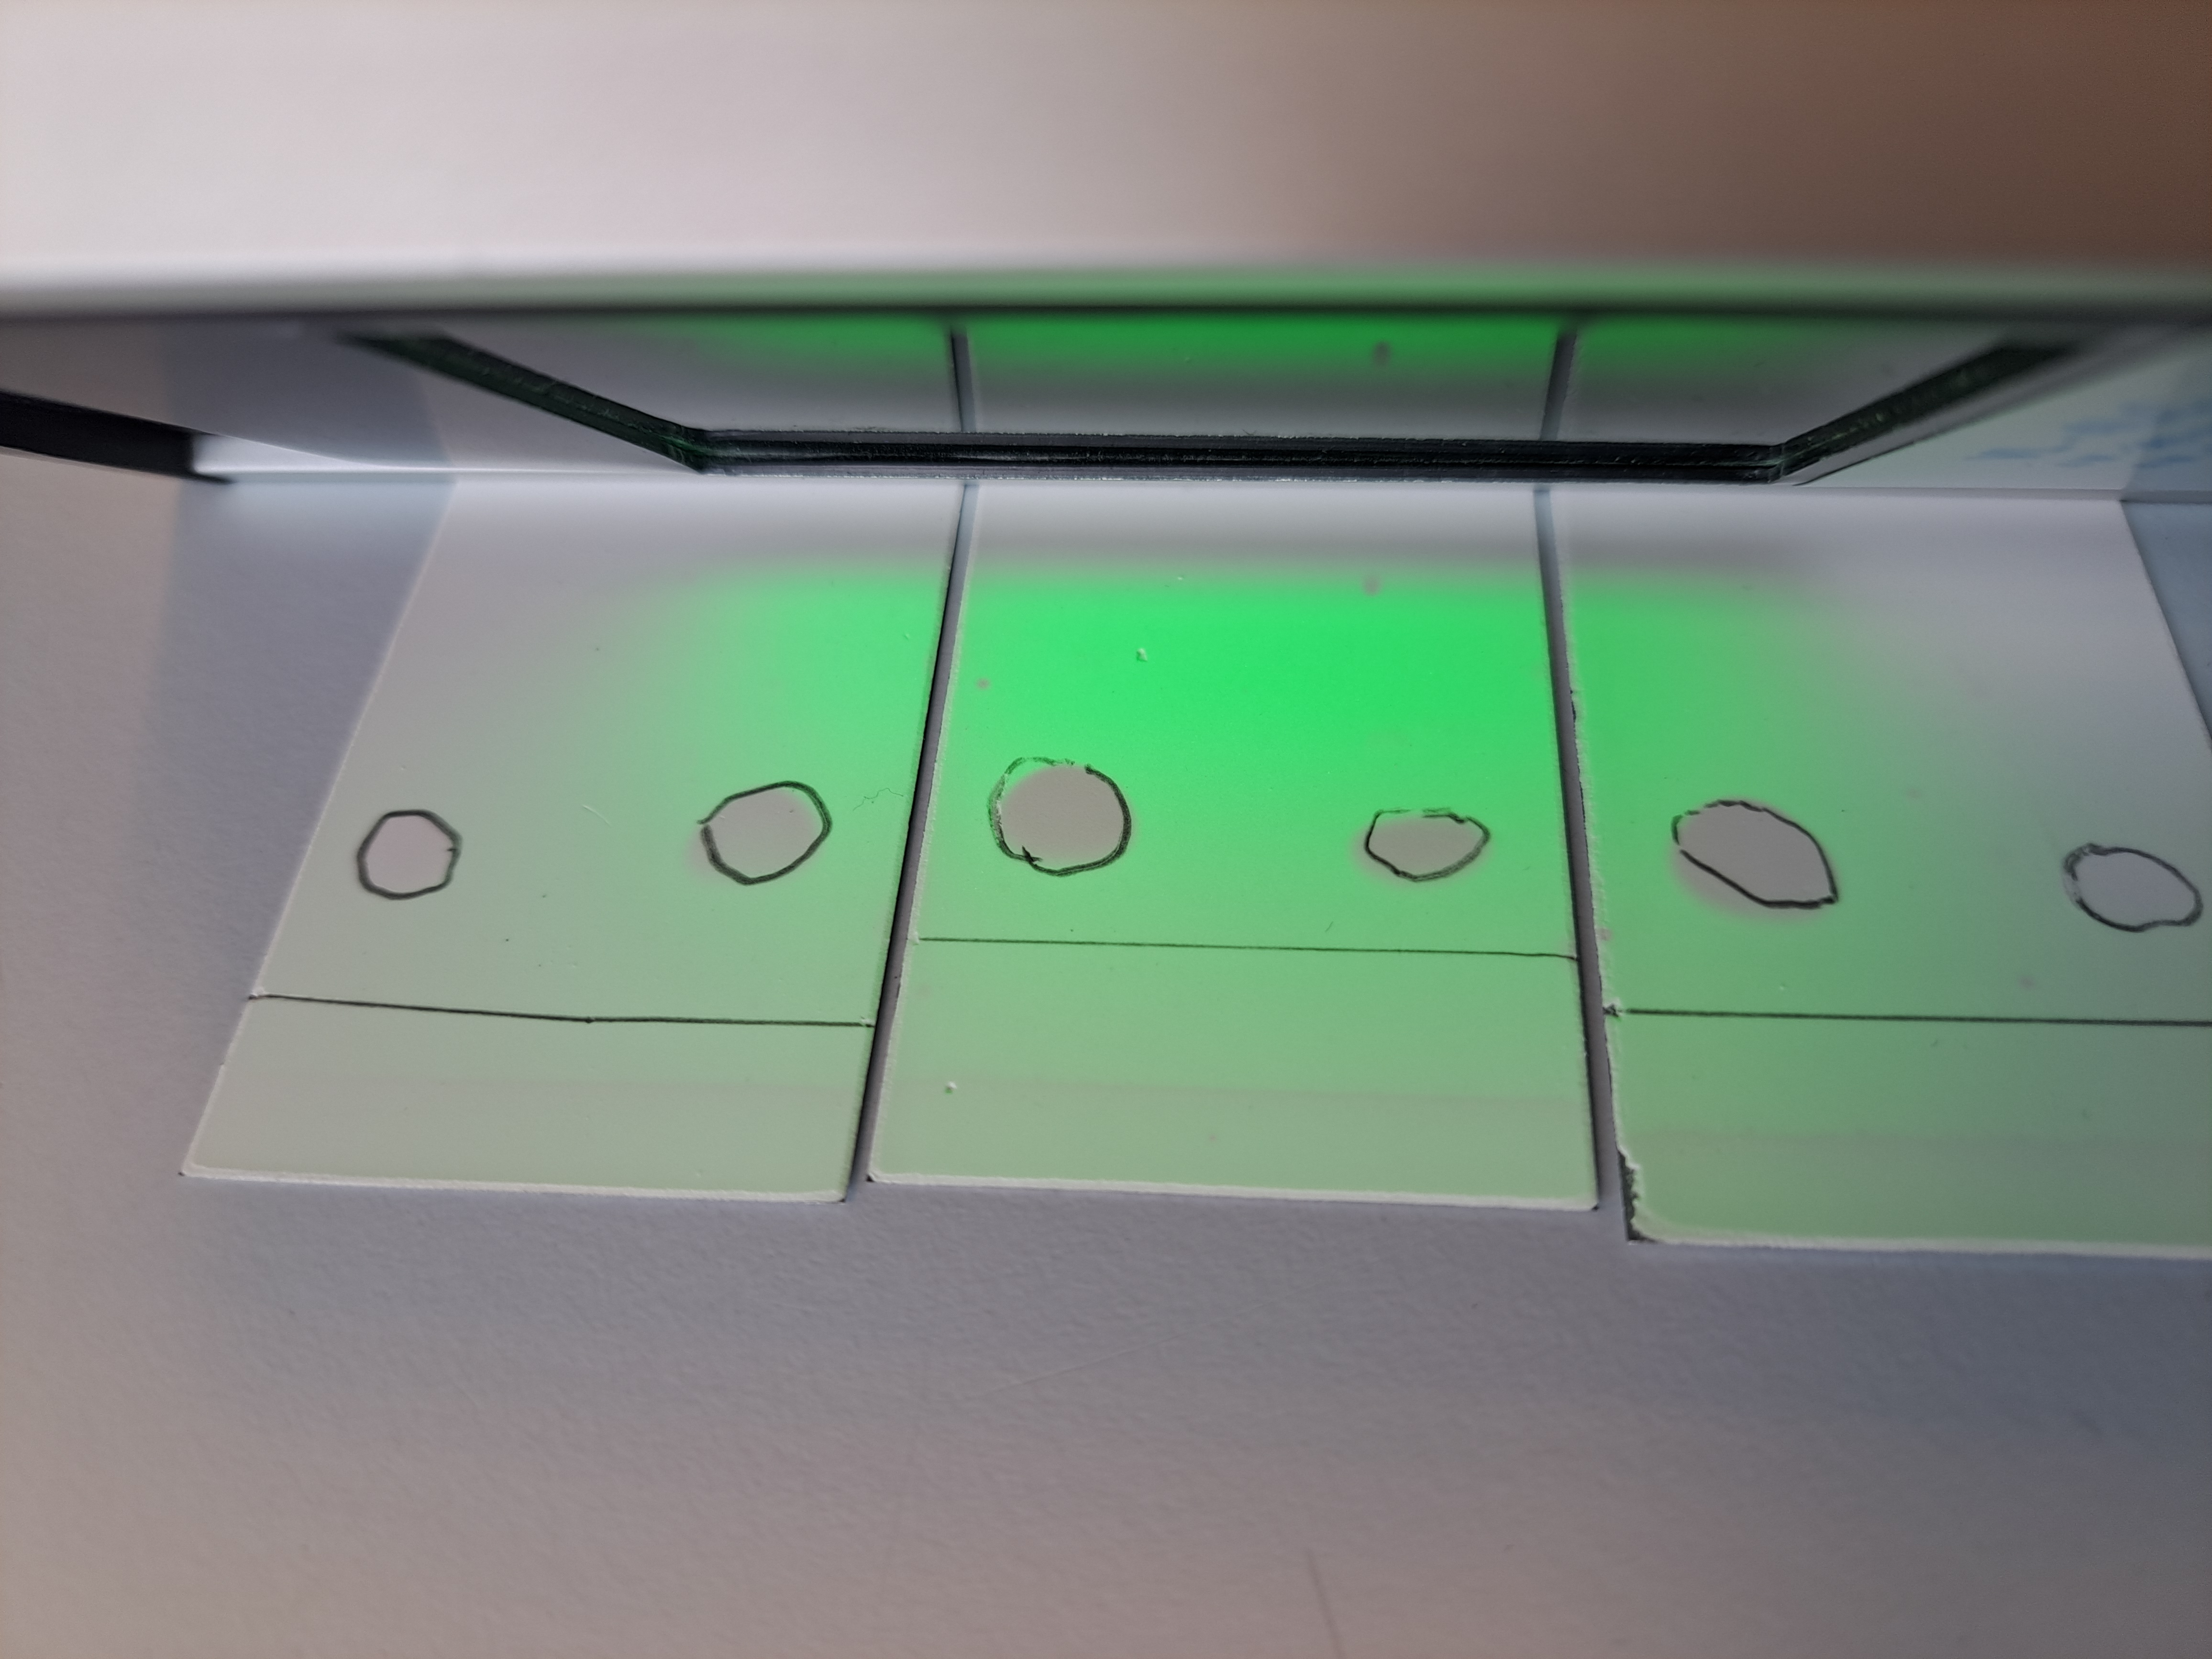
\includegraphics[width=0.48\linewidth]{billeder/tlc1}
        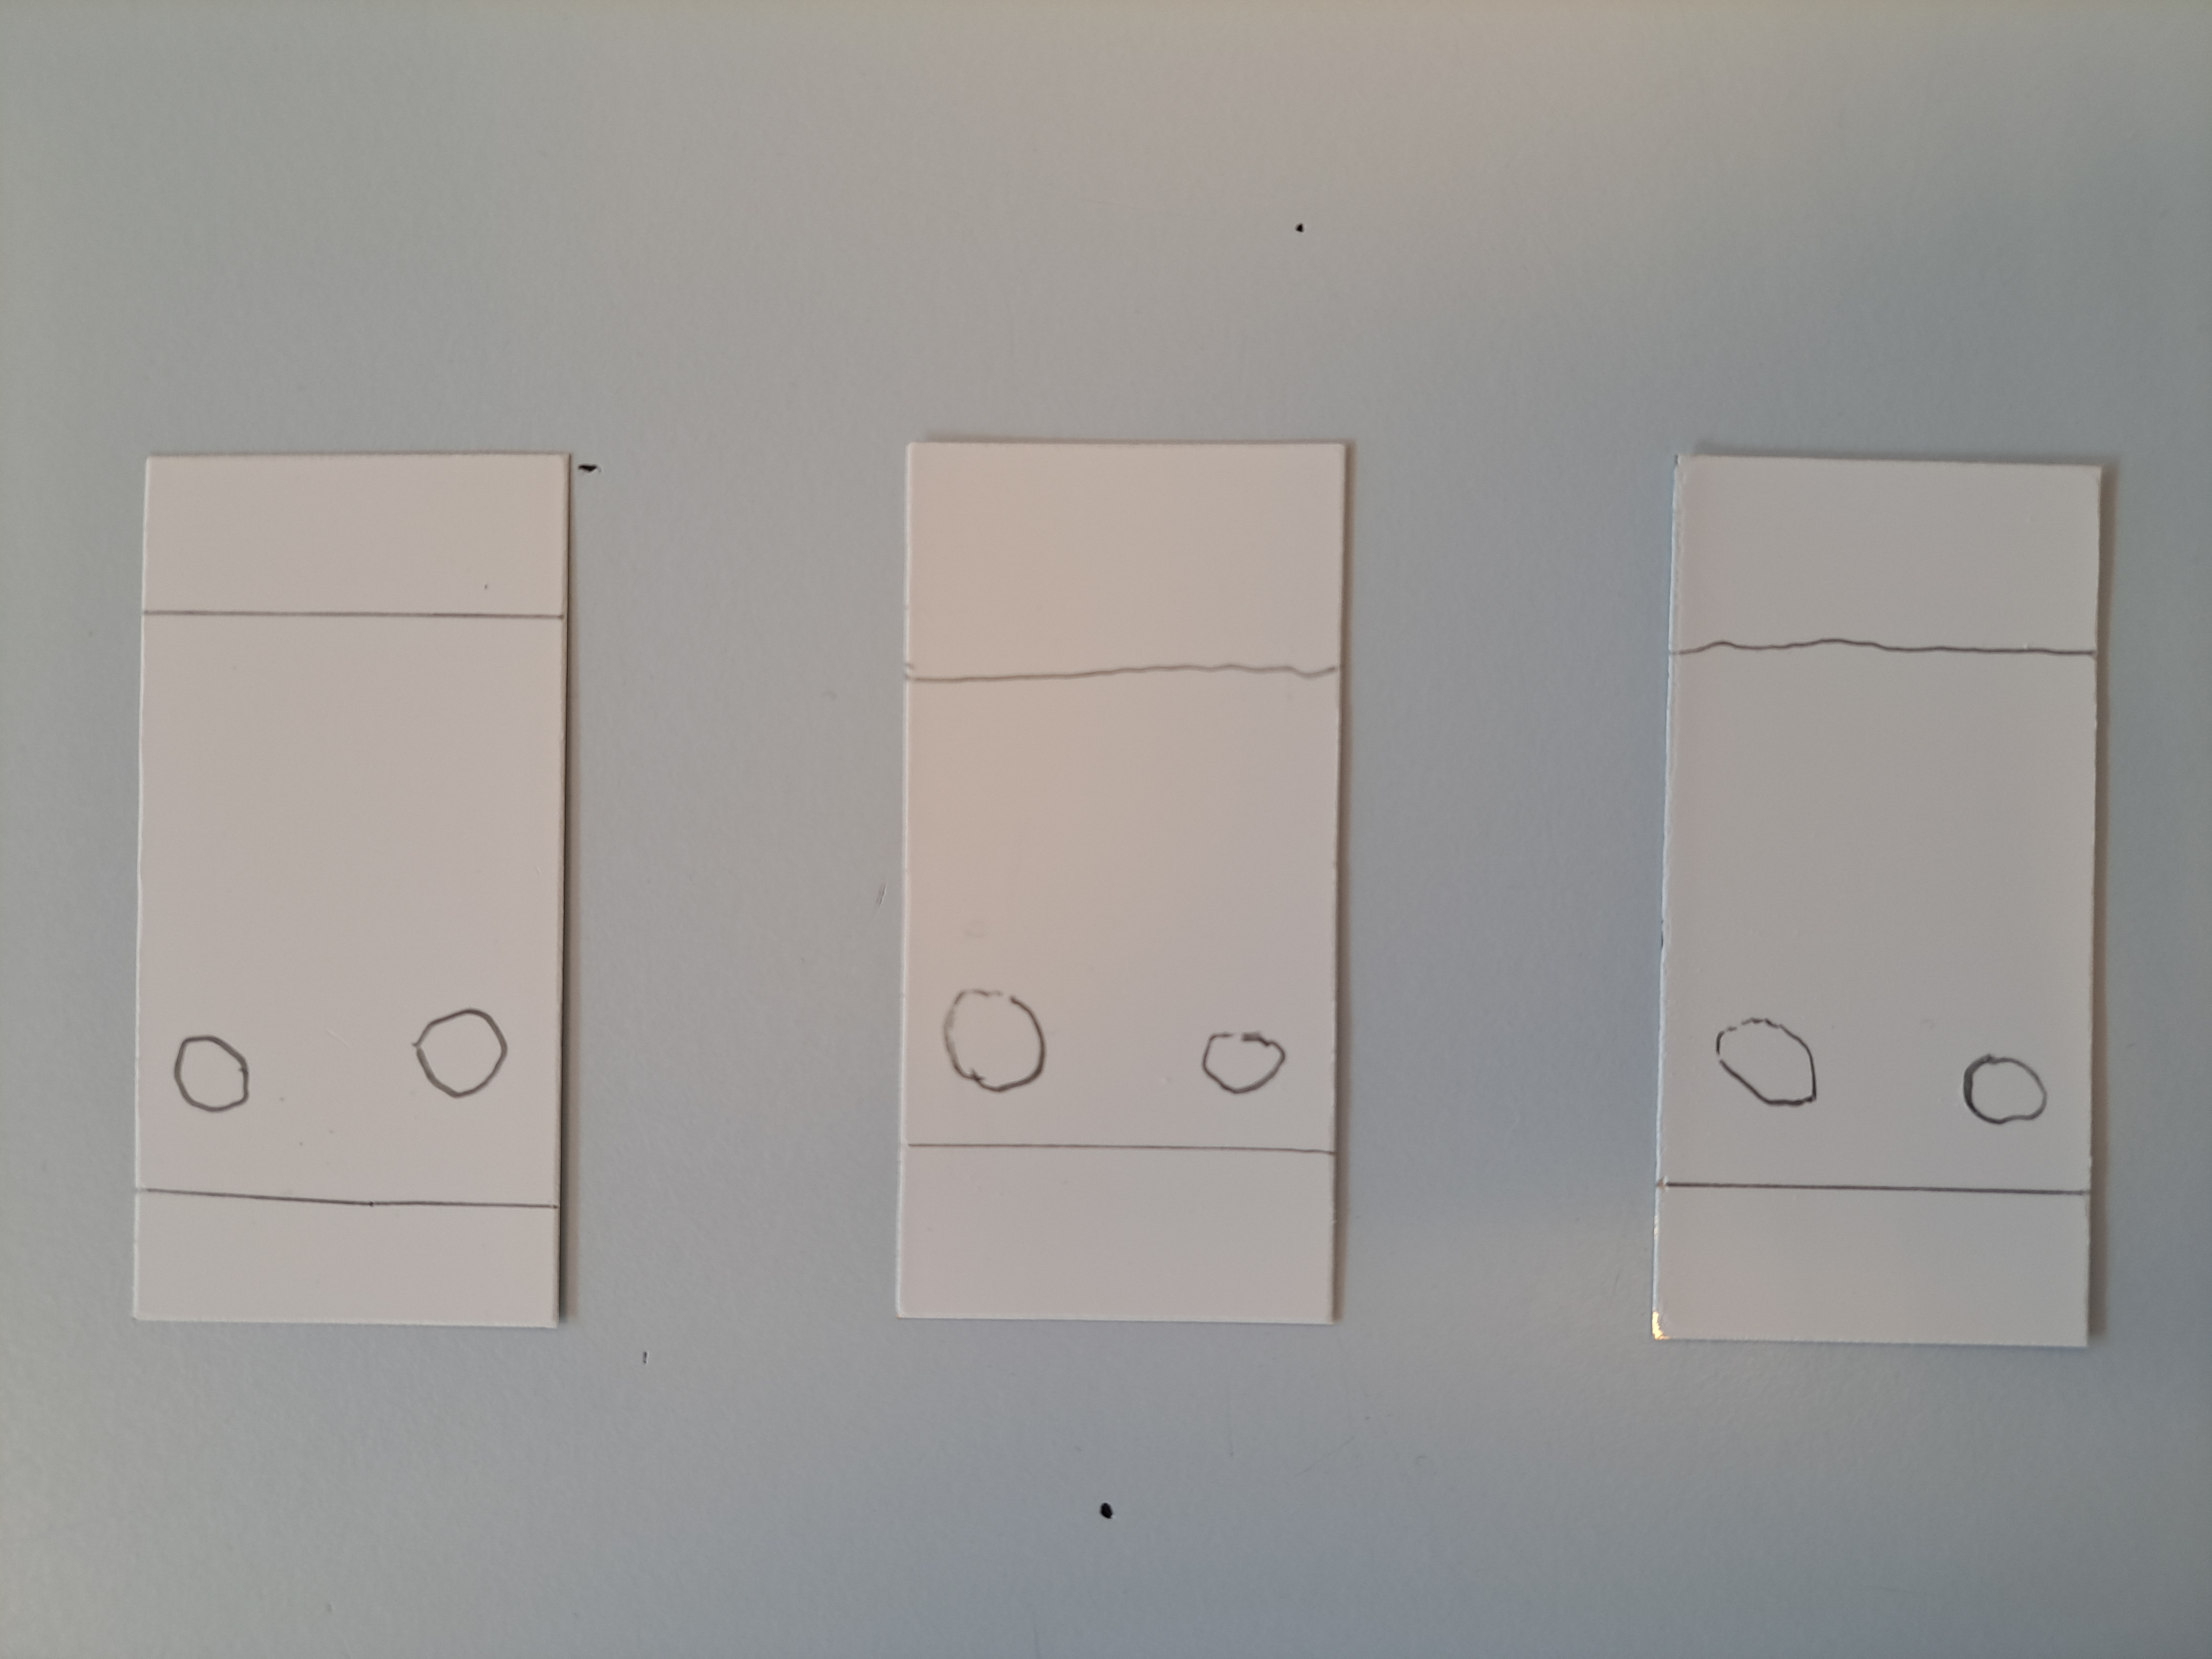
\includegraphics[width=0.48\linewidth]{billeder/tlcmarkeret1}
        \caption{TLC--plader fra syntese 1, eget produkt til venstre og kommercielt til højre}
    \end{figure} \vskip -24pt

    \subsection{Syntese 2}
    \begin{figure}[H]
        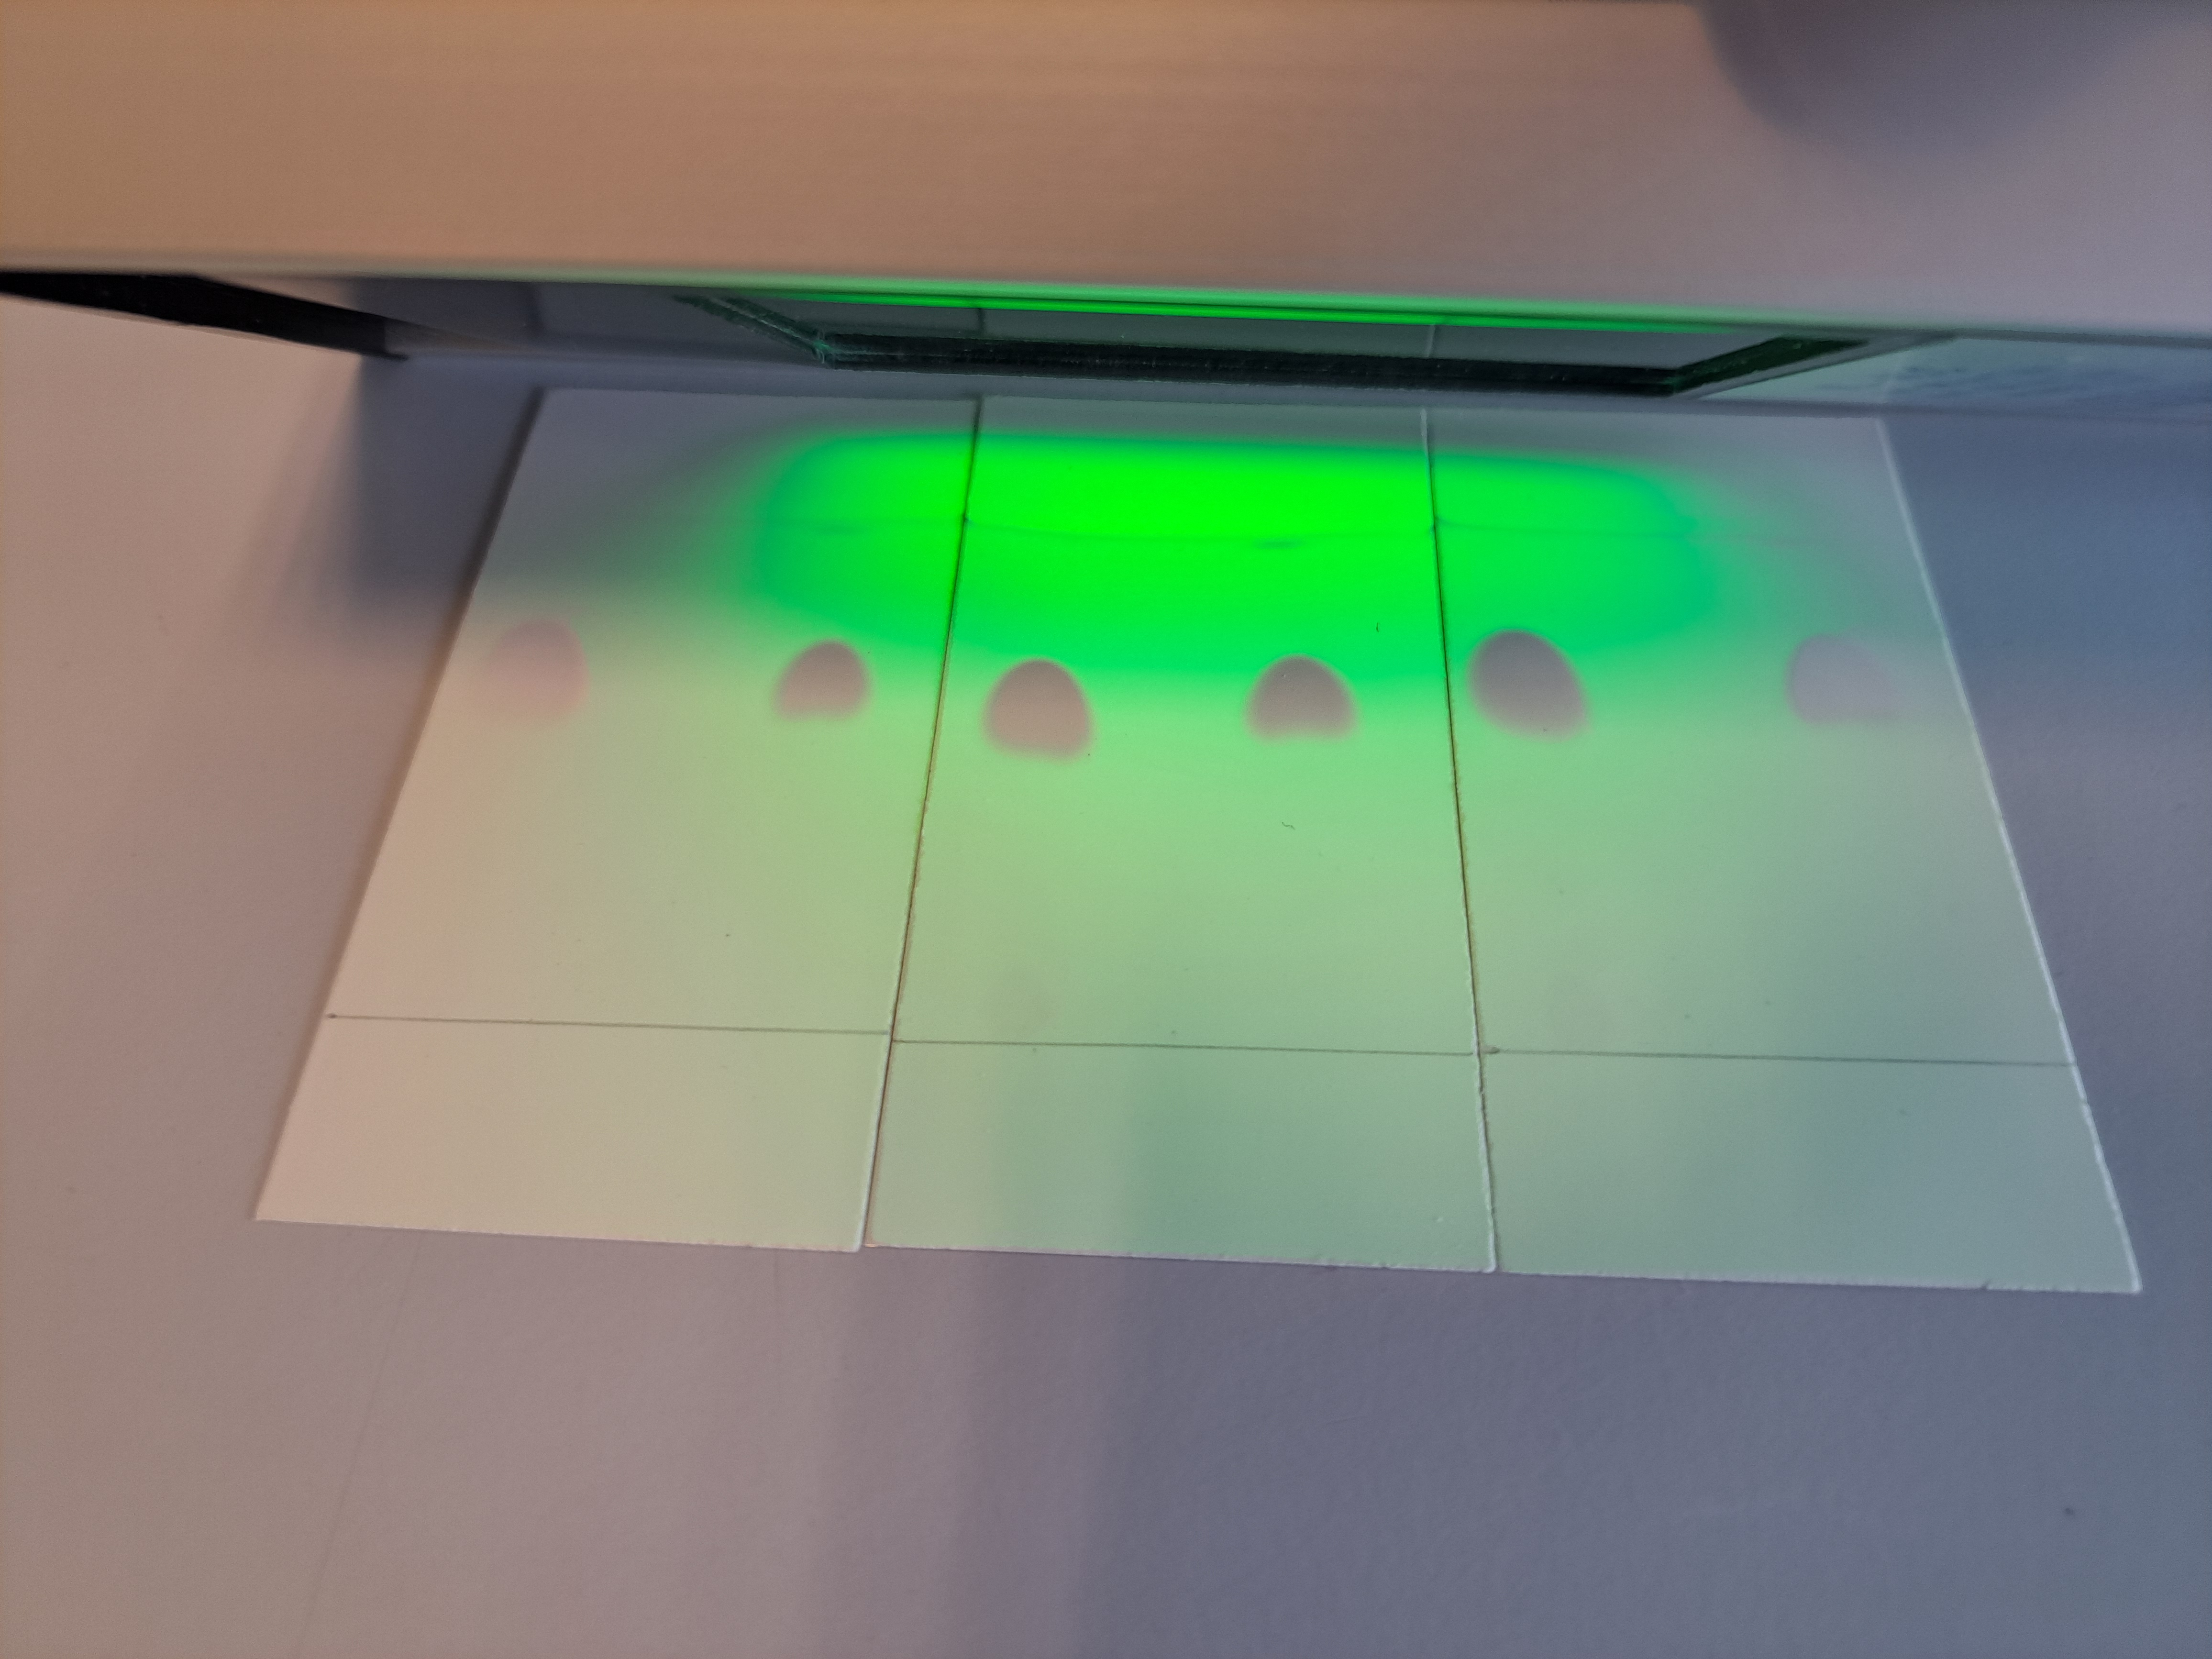
\includegraphics[width=0.48\linewidth]{billeder/tlc2}
        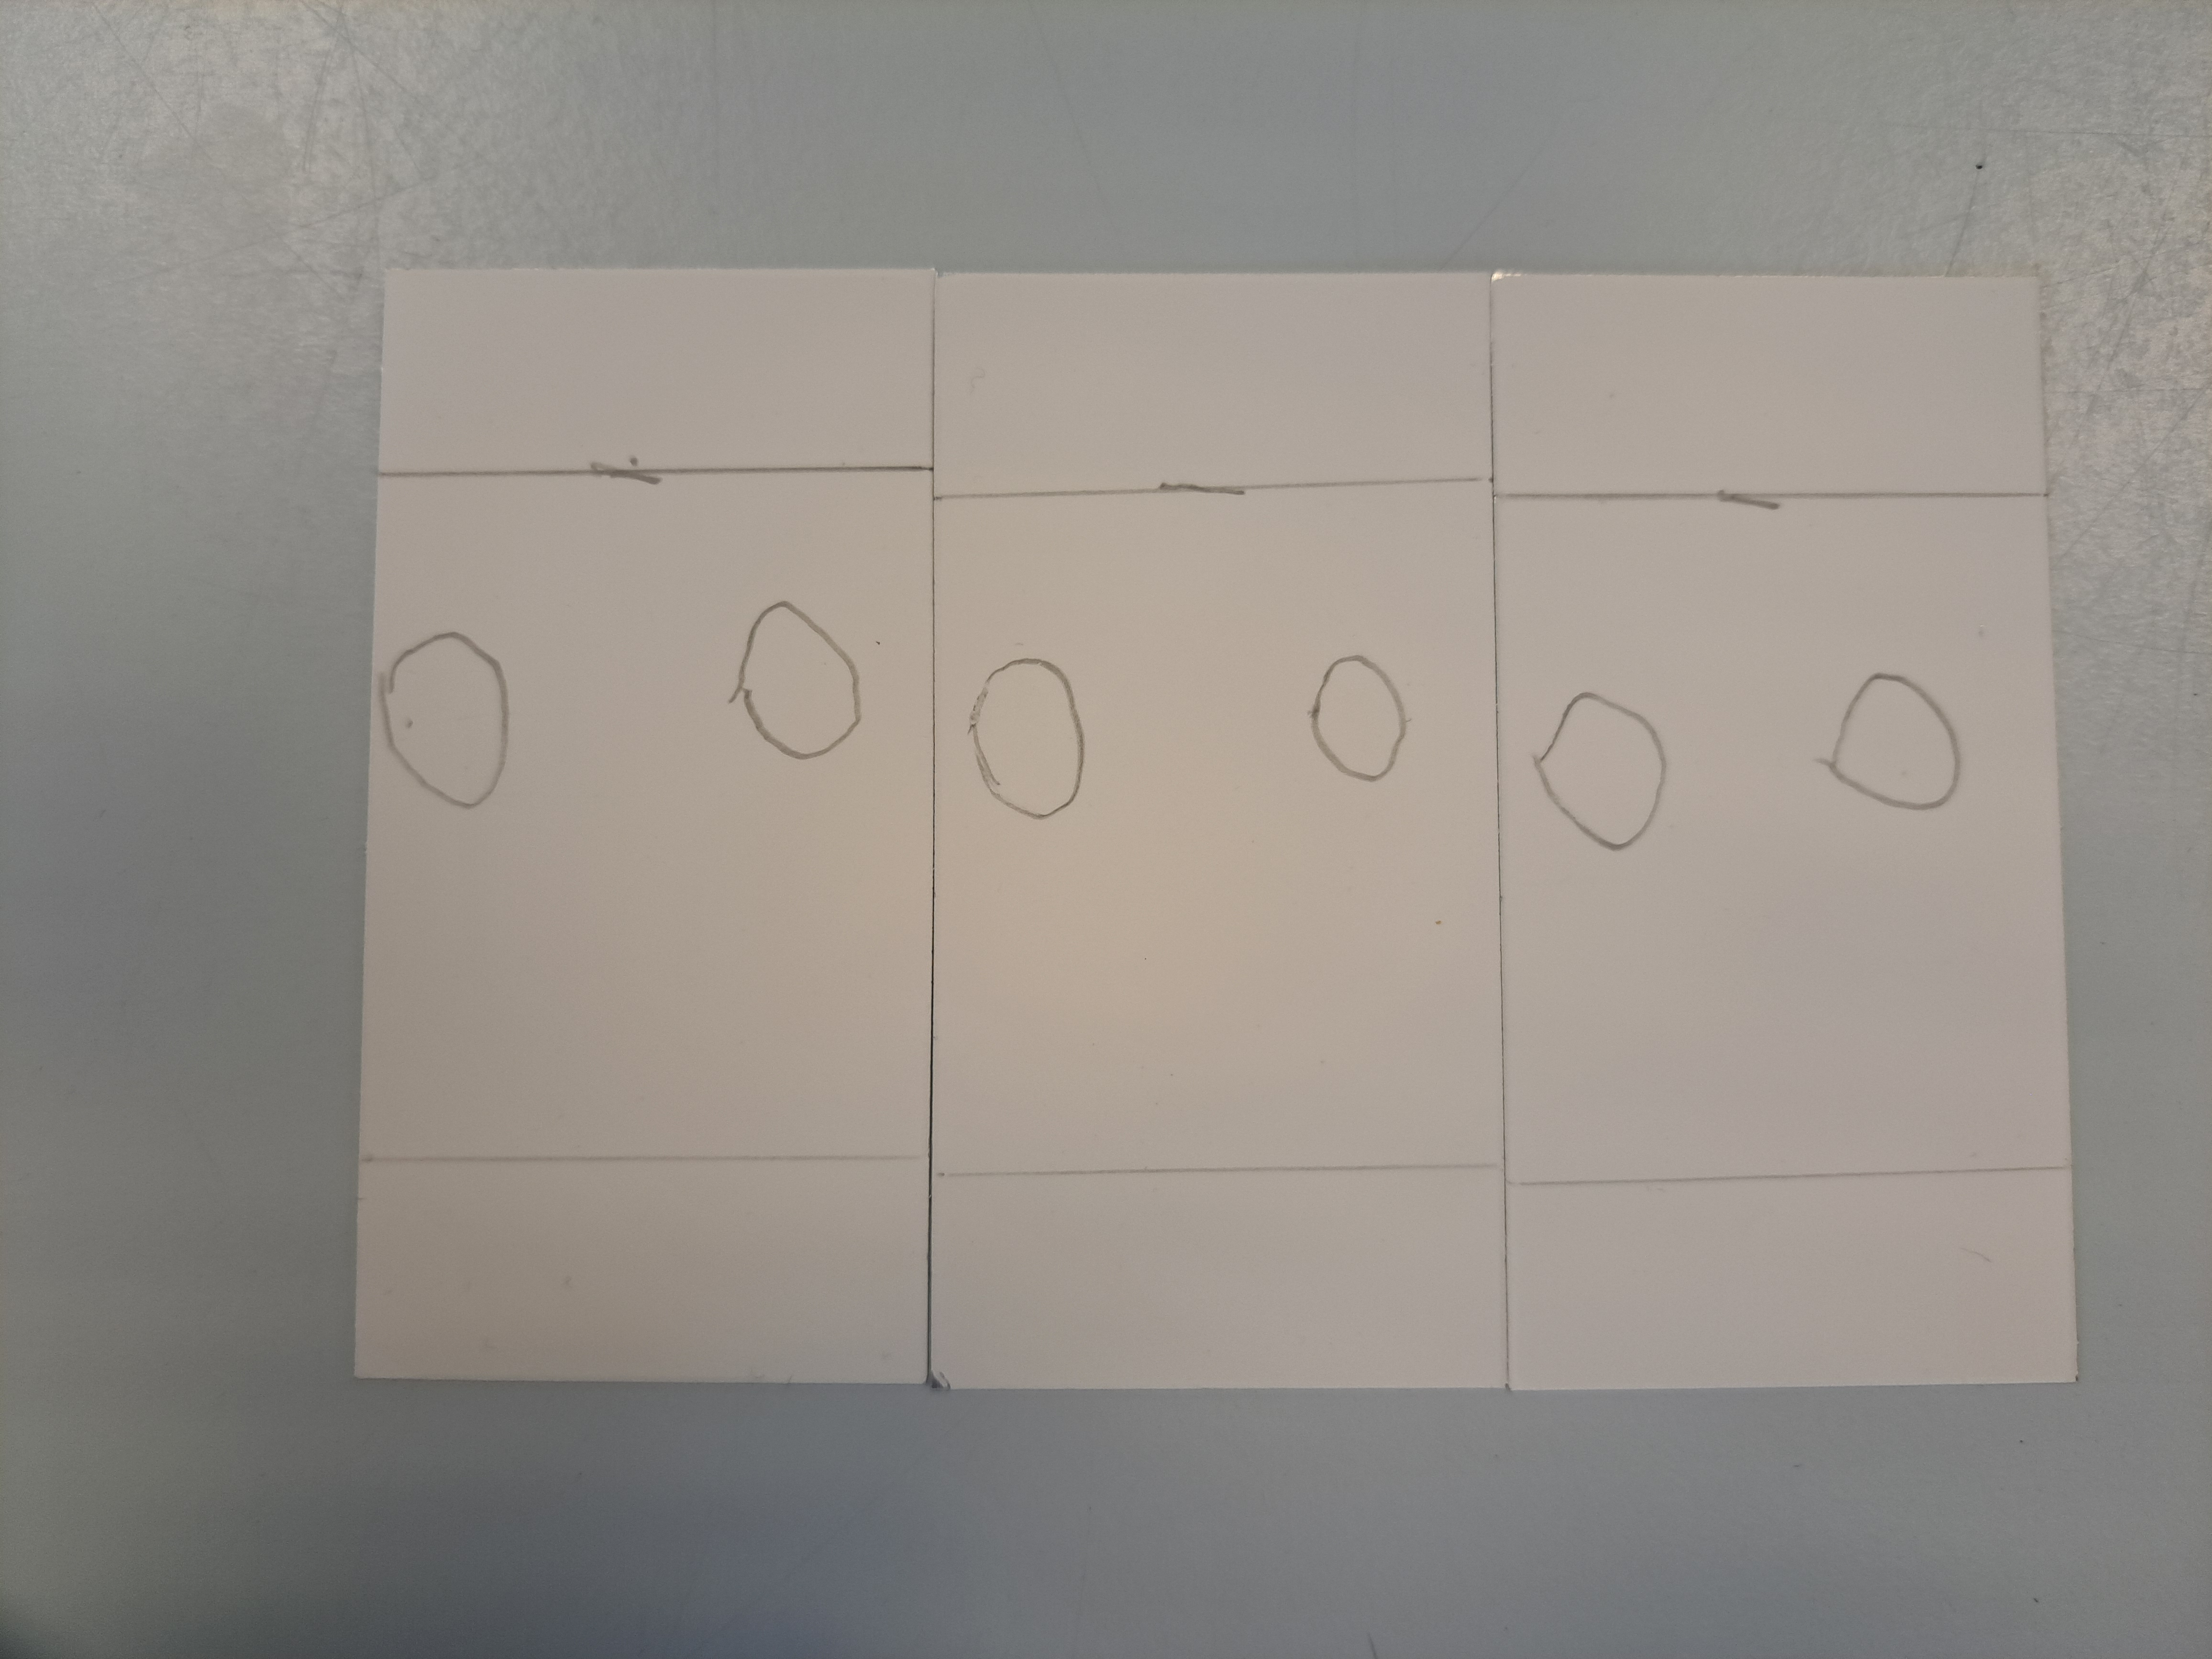
\includegraphics[width=0.48\linewidth]{billeder/tlcmarkeret2}
        \caption{TLC--plader fra syntese 2, eget produkt til venstre og kommercielt til højre}
    \end{figure} \vskip -24pt

    \subsection{Dobbeltsyntese}
    \begin{figure}[H]
        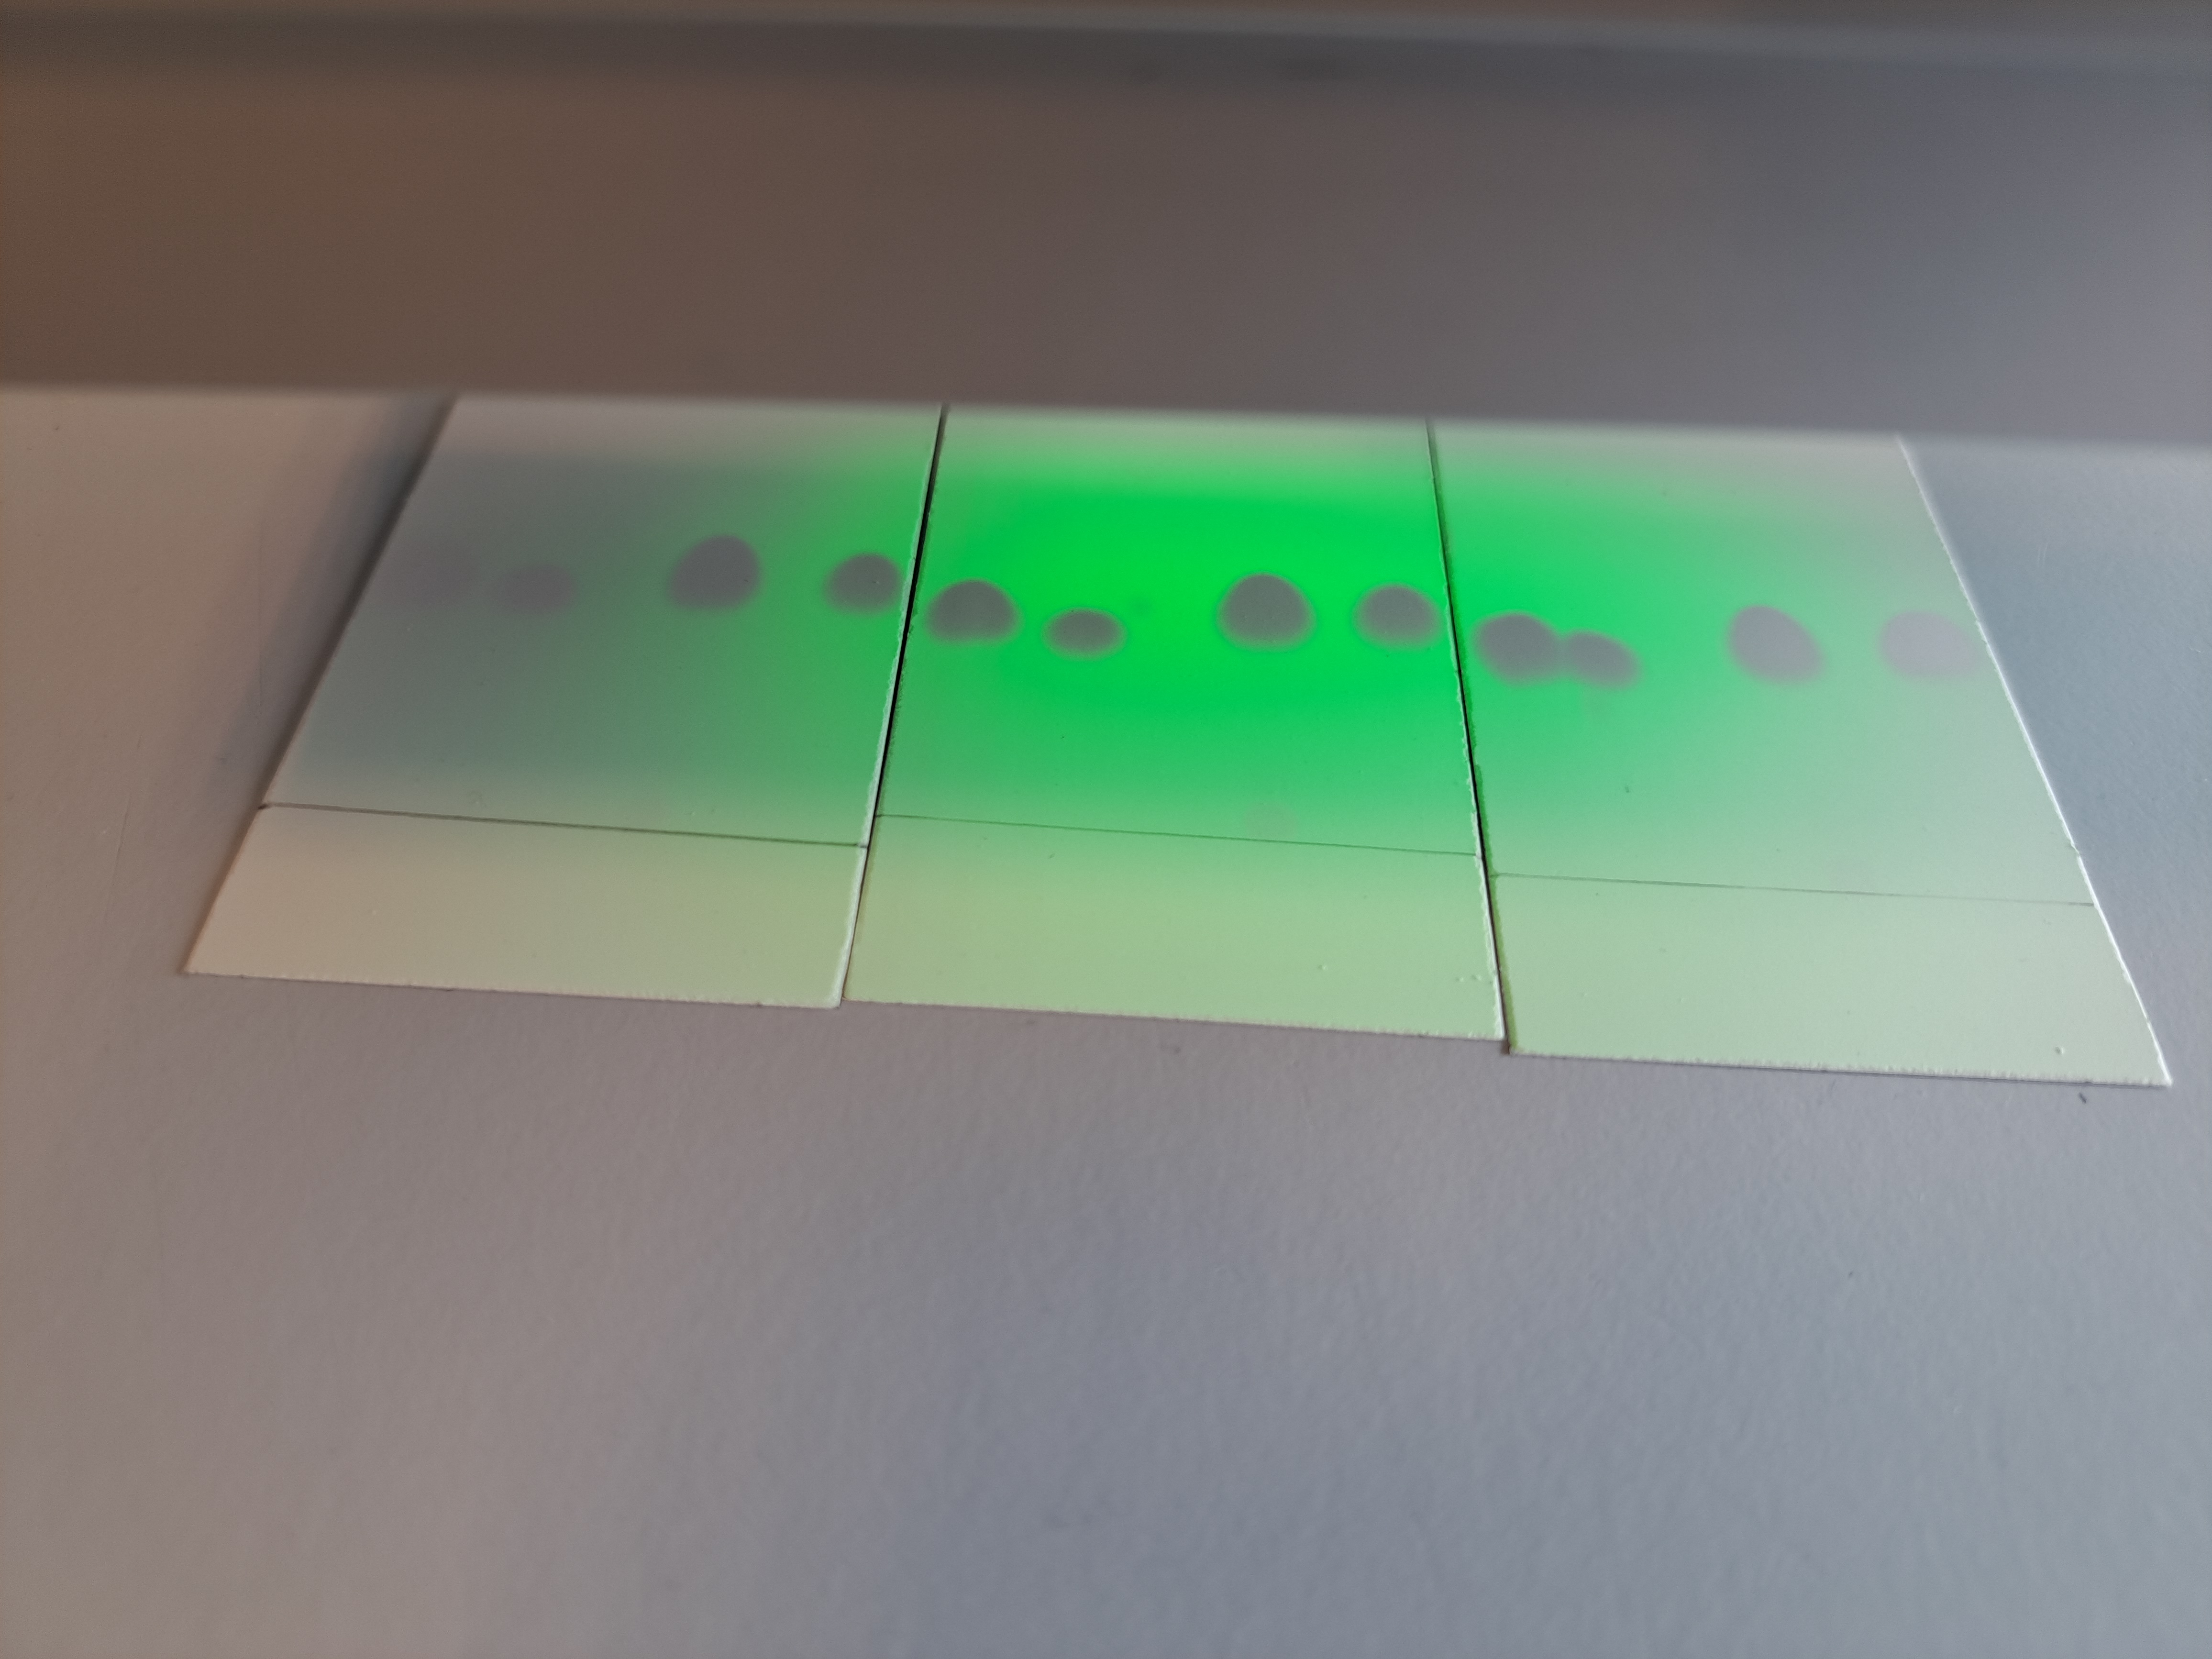
\includegraphics[width=0.48\linewidth]{billeder/tlc3}
        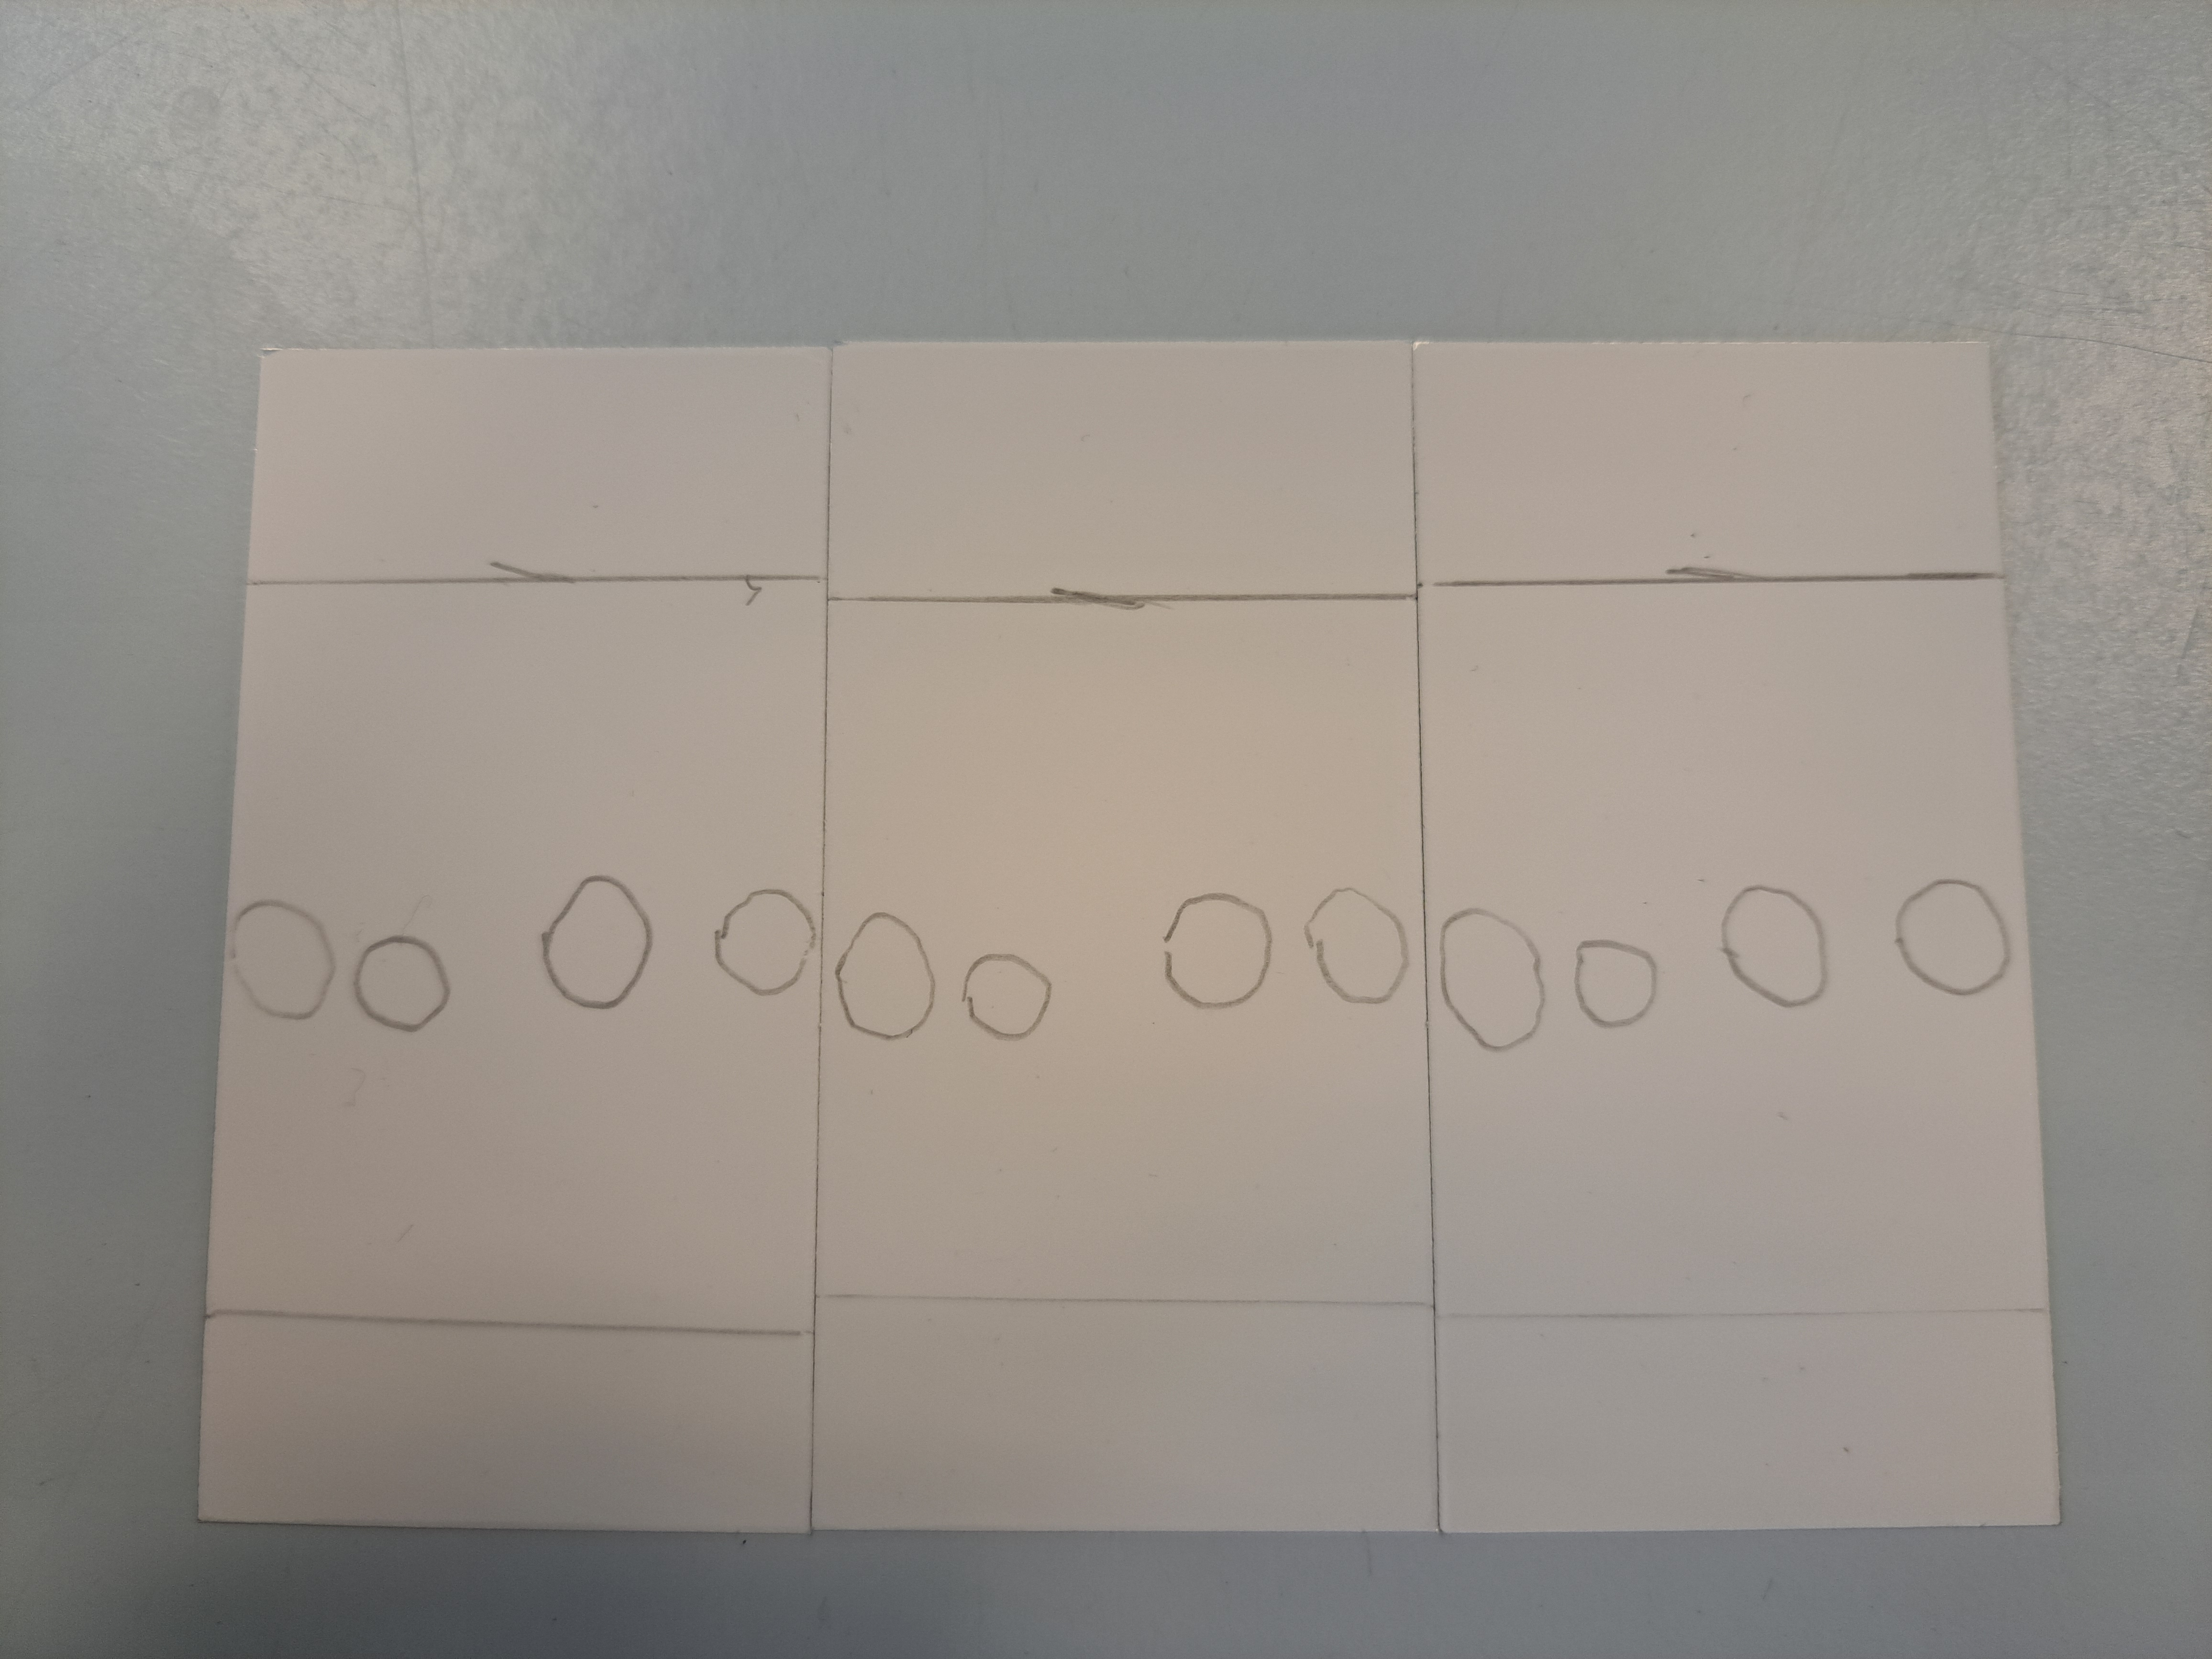
\includegraphics[width=0.48\linewidth]{billeder/tlcmarkeret3}
        \caption{TLC--plader fra syntese 3, første 2 er ethylparaben, næste 2 er propylparaben, eget produkt til venstre og kommercielt til højre}
    \end{figure} \vskip -24pt

    \captionsetup{font={color=white}}
    \addcontentsline{toc}{section}{H--NMR--Spektre}

    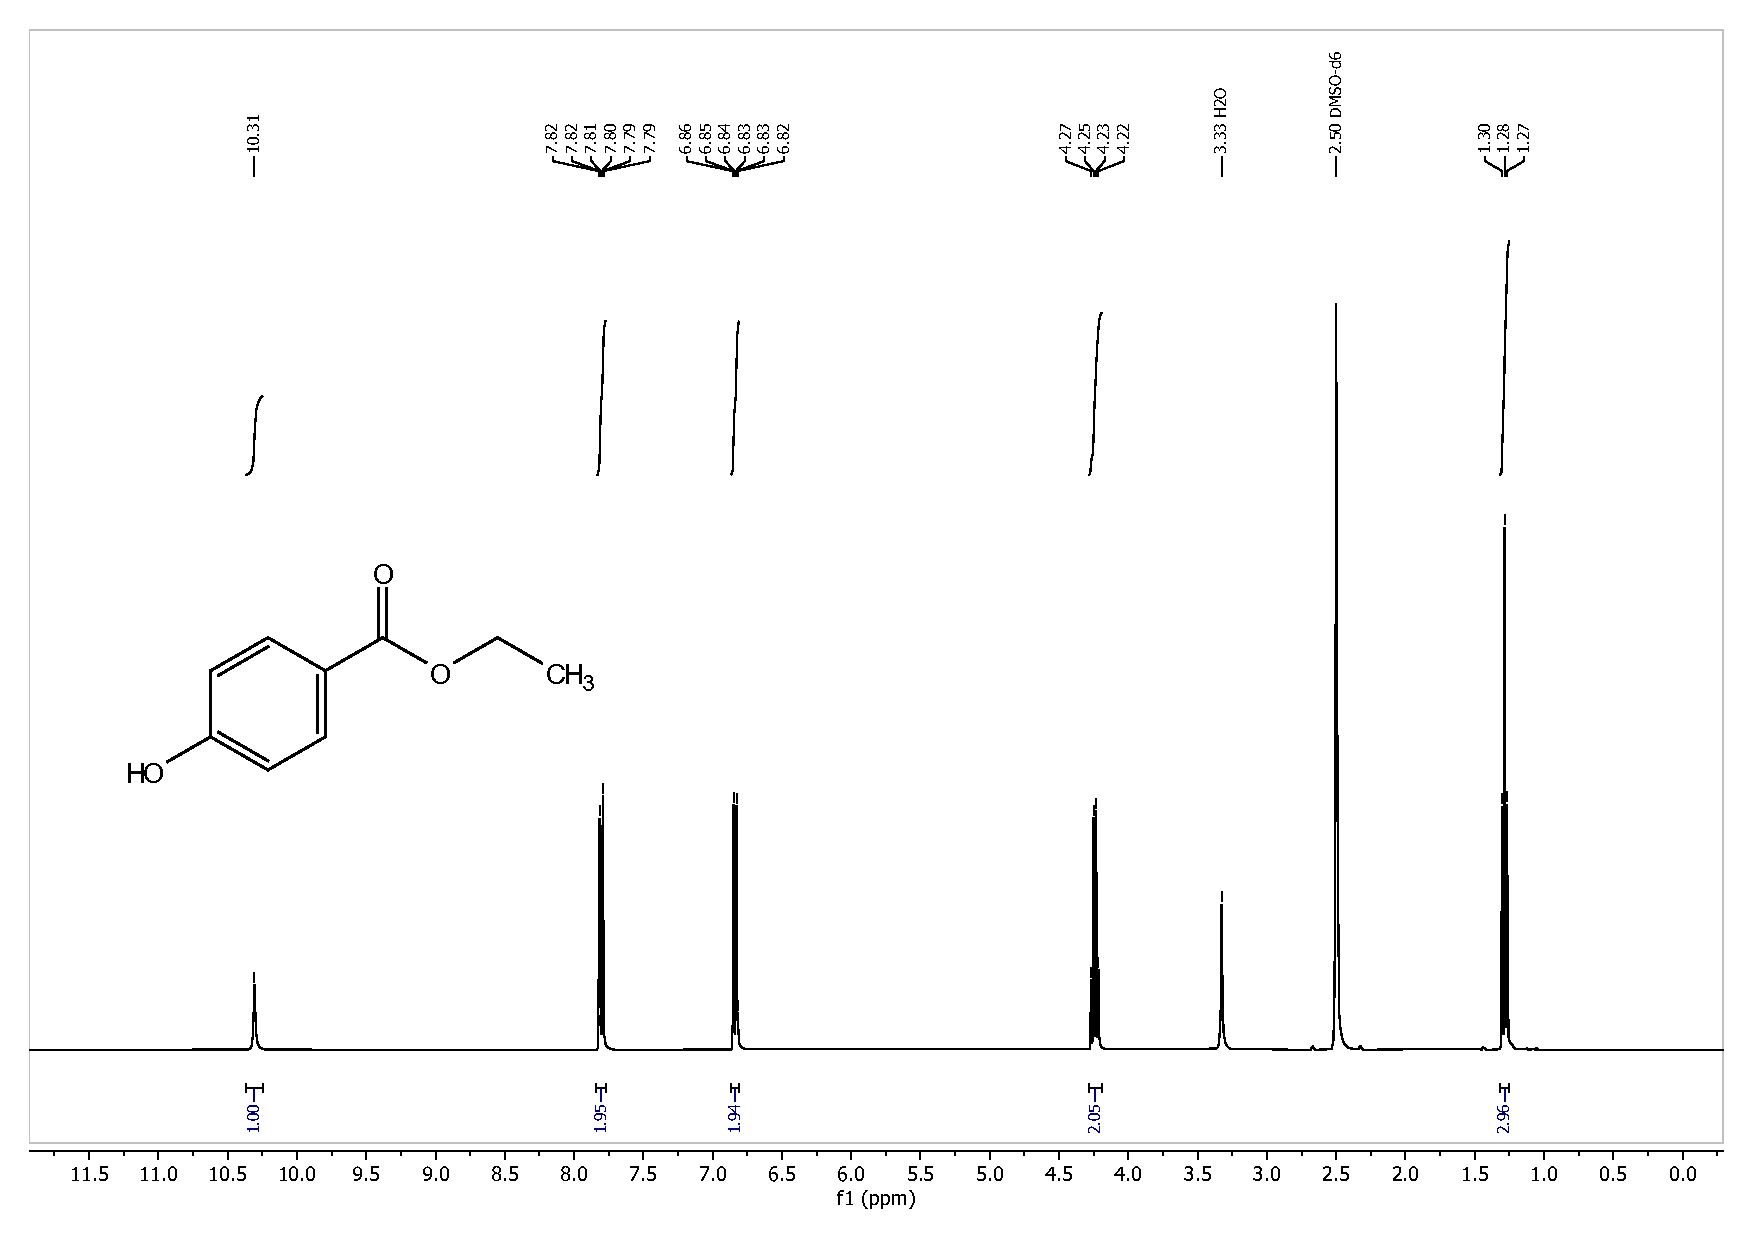
\includepdf[pages=-,landscape=true,addtotoc={1,subsection,2,Ethylparaben,ethylspek,2,subsubsection,3,Peaks,ethylpeaks}]{bilag/ethylnmr.pdf}

    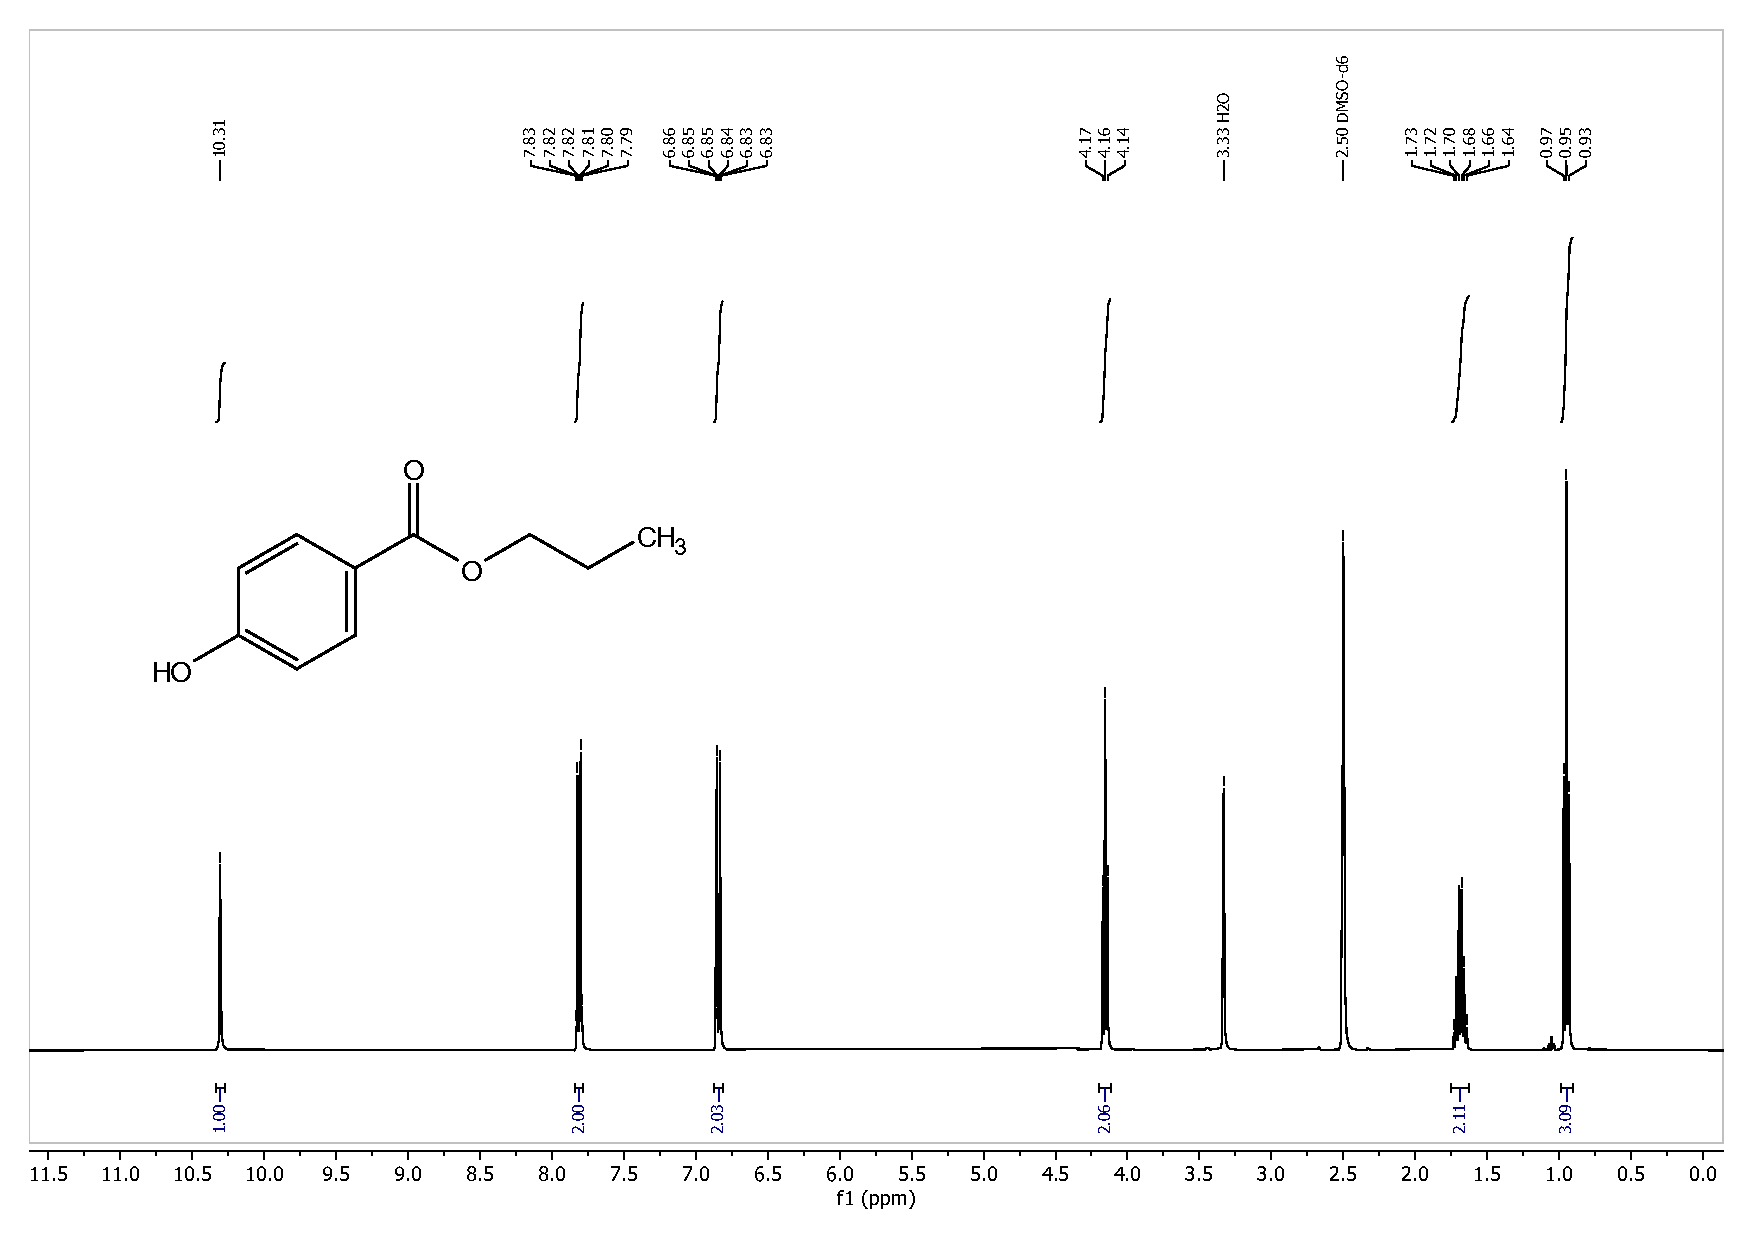
\includepdf[pages=-,landscape=true,addtotoc={1,subsection,2,Propylparaben,propylspek,2,subsubsection,3,Peaks,propylpeaks}]{bilag/propylnmr.pdf}

    \addcontentsline{toc}{section}{IR--Spektre}

    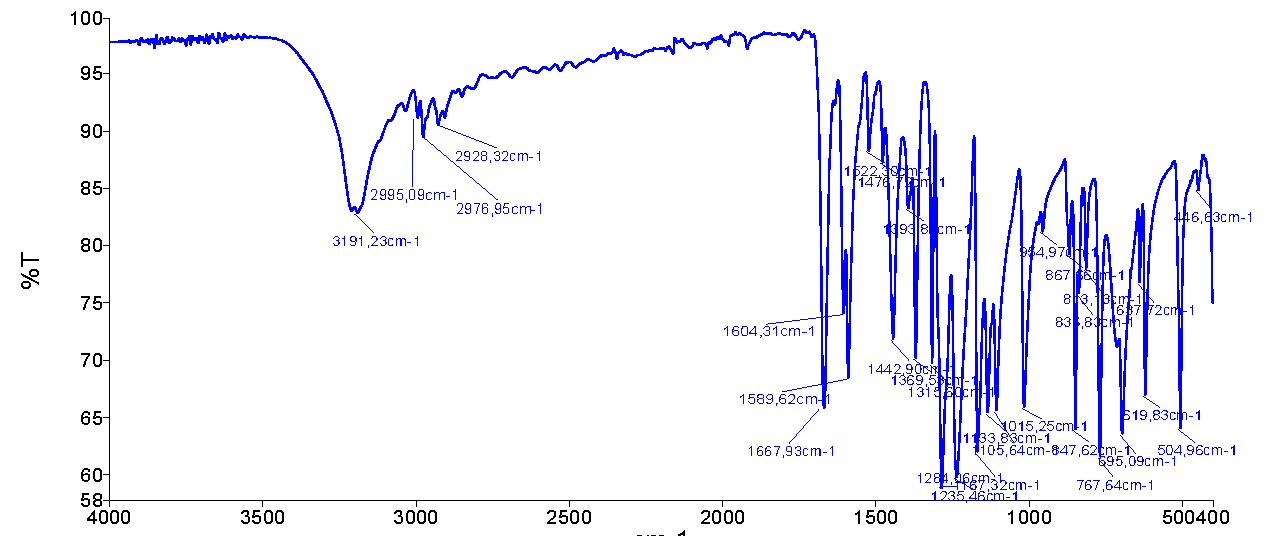
\includepdf[pages=-,landscape=true,addtotoc={1,subsection,1,Ethylparaben,ethylir}]{bilag/ethylir.pdf}

    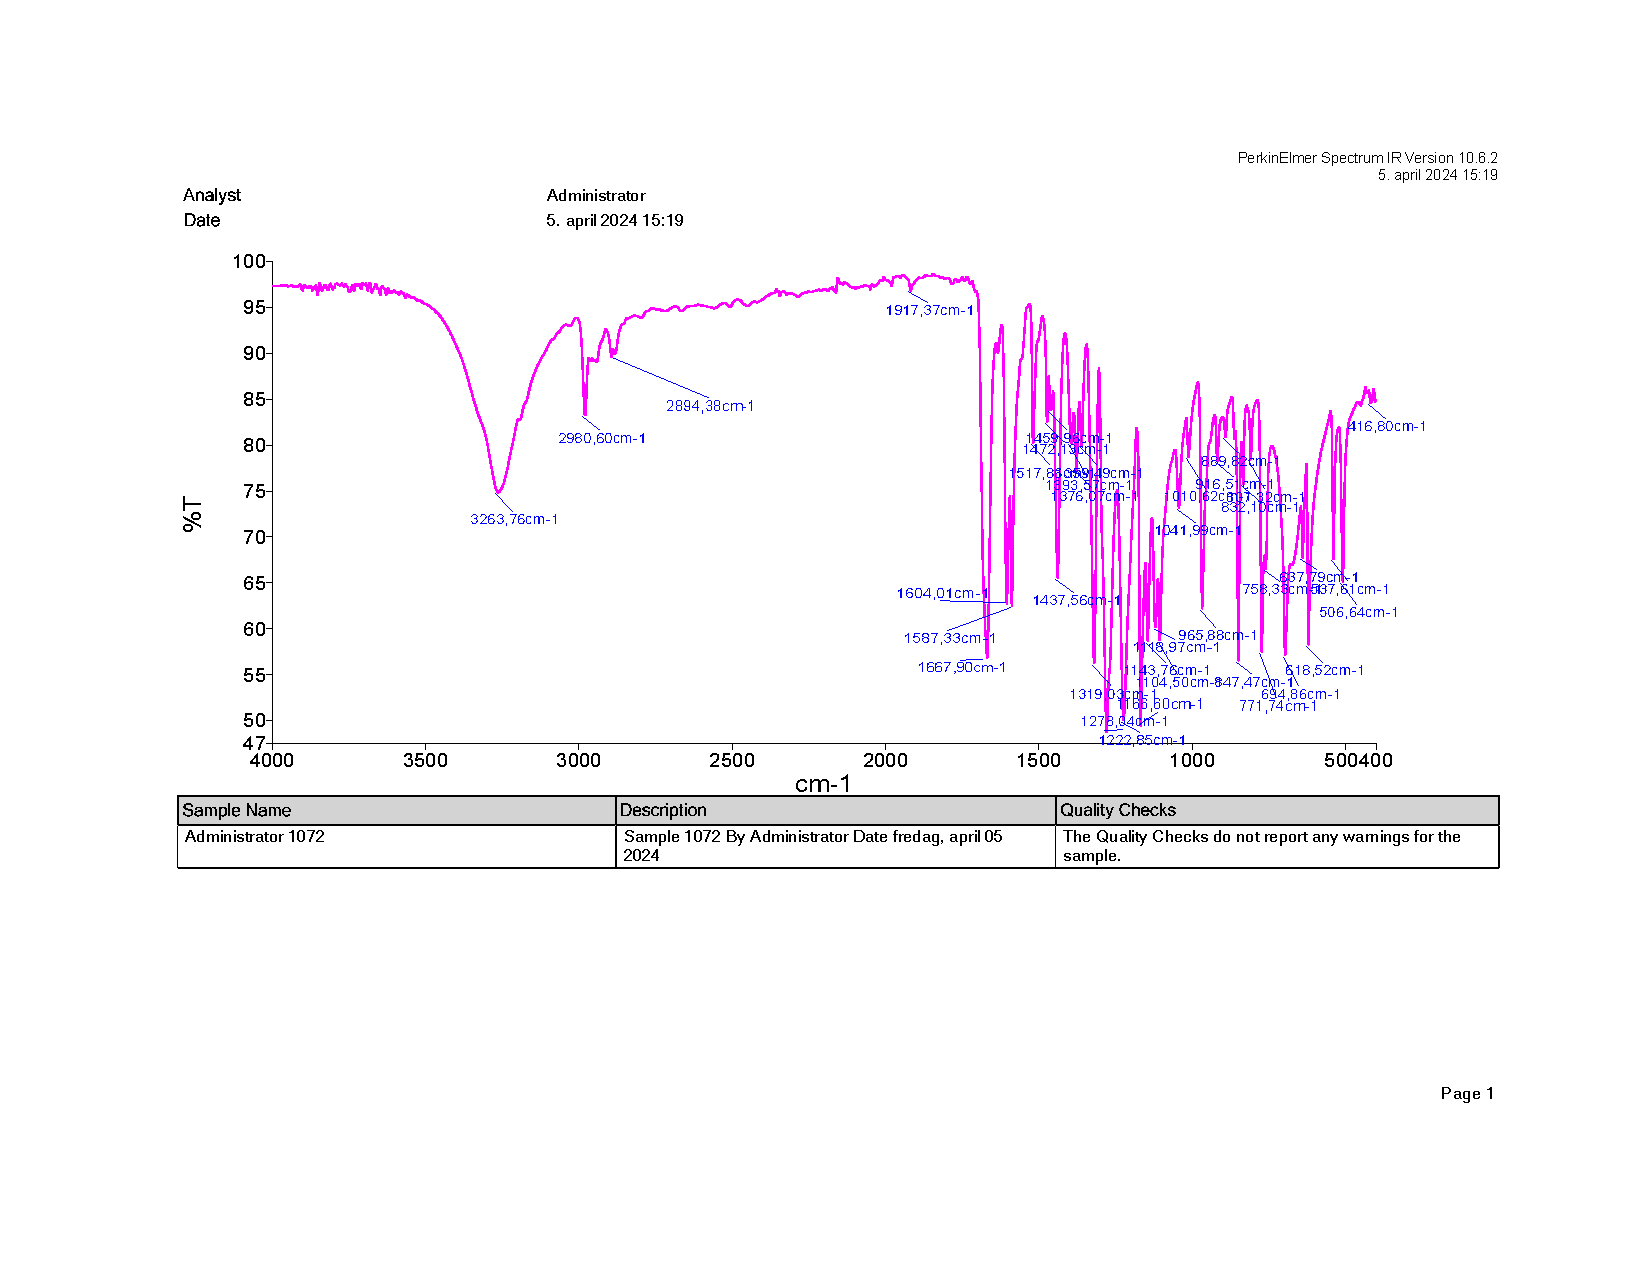
\includepdf[pages=-,landscape=true,addtotoc={1,subsection,1,Propylparaben,propylir}]{bilag/propylir.pdf}

    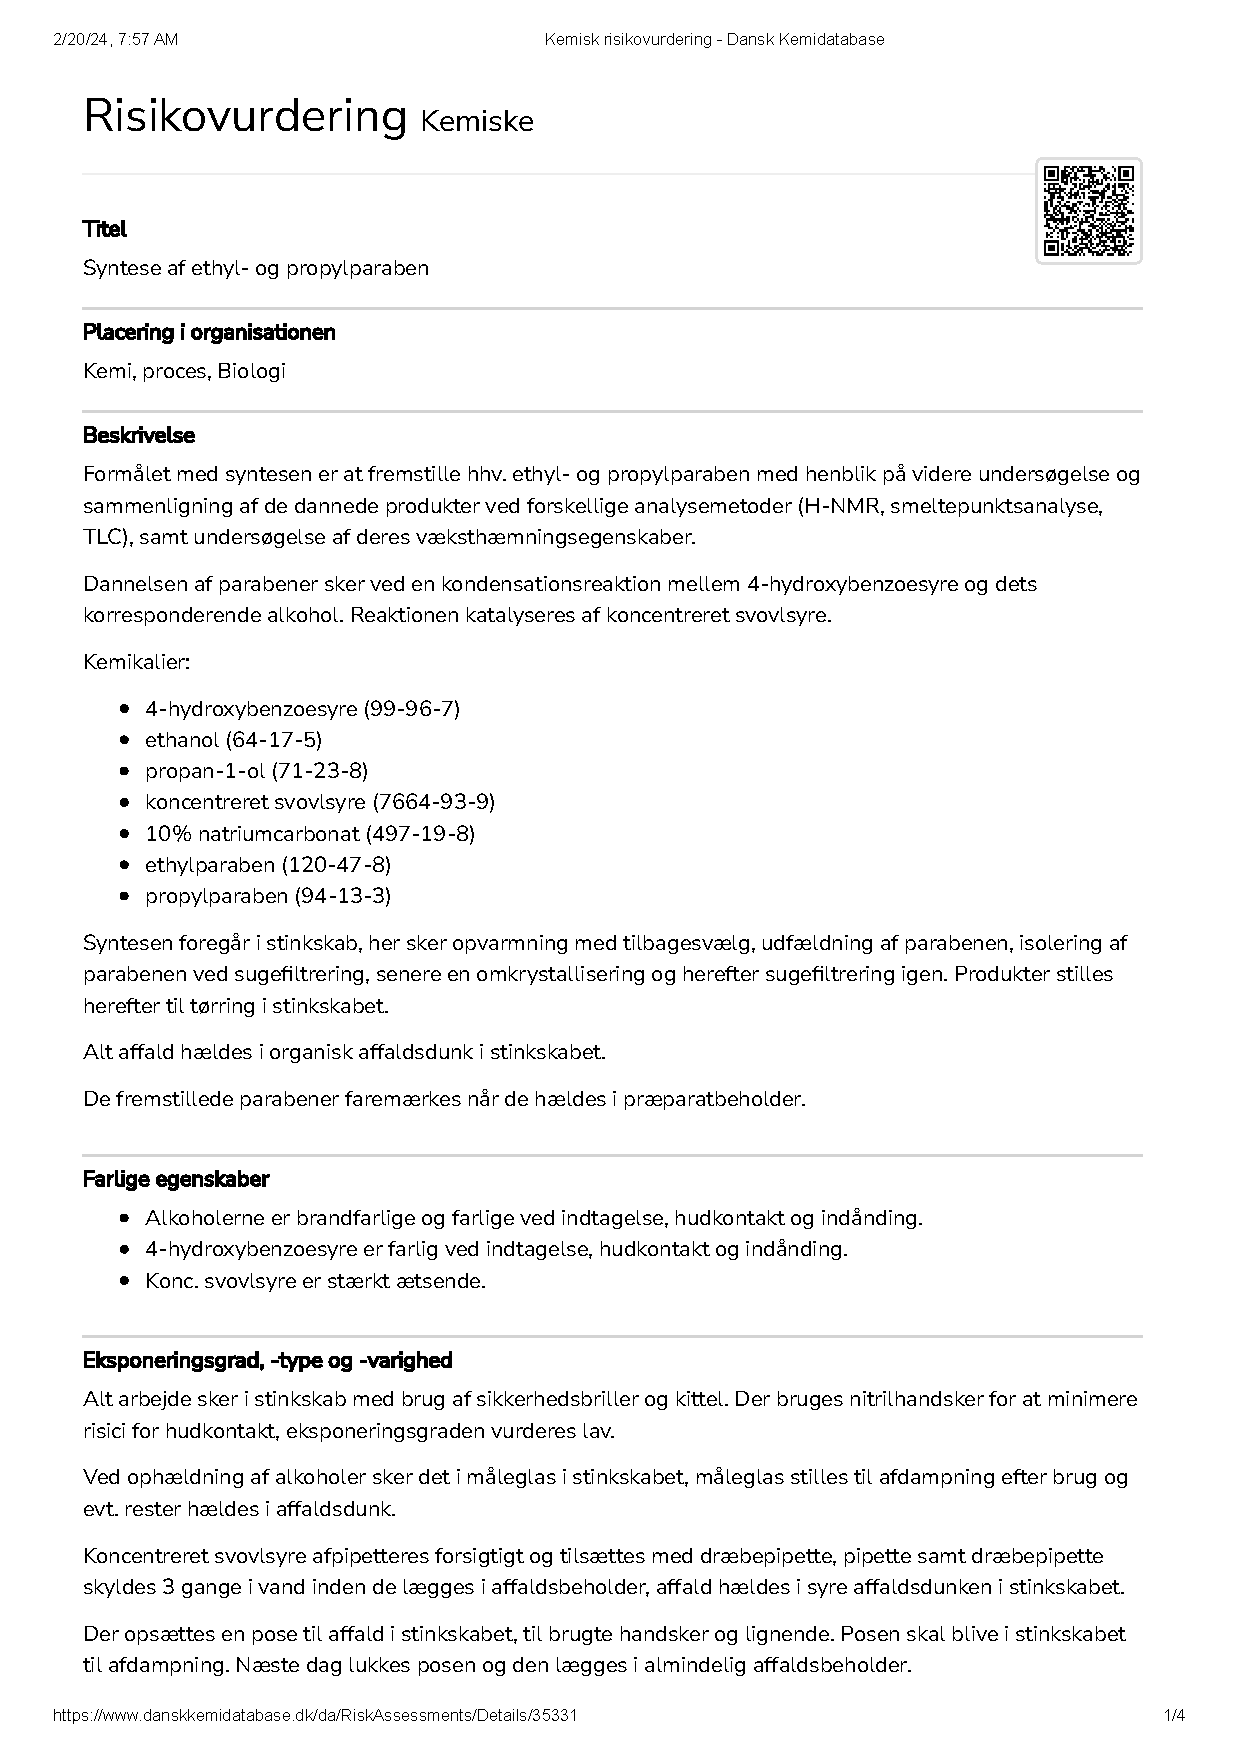
\includepdf[pages={1,2,3},addtotoc={1,section,1,Risikovurdering,risikovurdering}]{bilag/risikovurdering.pdf}
